\documentclass[a4paper, 12pt]{article}


\usepackage[french]{babel}
\usepackage[utf8]{inputenc}
\usepackage[T1]{fontenc}
\usepackage{lmodern}
\usepackage{listings}
\usepackage{graphicx}
\usepackage{amsmath}
\usepackage{amsfonts}
\usepackage{amssymb}
\usepackage{caption}
\usepackage{subcaption}
\usepackage[usenames,dvipsnames]{xcolor}


\setcounter{secnumdepth}{4}
% TAILLE DES PAGES (A4 serré)

\setlength{\parindent}{0pt}
\setlength{\parskip}{1ex}
\setlength{\textwidth}{17cm}
\setlength{\textheight}{24cm}
\setlength{\oddsidemargin}{-.7cm}
\setlength{\evensidemargin}{-.7cm}
\setlength{\topmargin}{-.5in}

% Commandes de mise en page
\newcommand{\fichier}[1]{\emph{#1}}
\newcommand{\nom}[1]{\emph{#1}}
\newcommand{\Fig}[1]{Fig \ref{#1} p. \pageref{#1}}
\newcommand{\itemi}{\item[$\bullet$]}

% Commandes de maths
\newcommand{\fonction}[3]{#1 : #2 \to #3}
\newcommand{\intr}[2]{\left[ #1 ; #2 \right]}
\newcommand{\intn}[2]{\left[\![ #1 ; #2 \right]\!]}
\newcommand{\intro}[2]{\left] #1 ; #2 \right[}
\newcommand{\intrsod}[2]{\left[ #1 ; #2 \right[}
\newcommand{\ps}[2]{\langle #1, #2 \rangle}
\newcommand{\mdelta}[1]{\boldsymbol{\delta_{#1}}}
%% \newcommand{\mdelta}[1]{\delta_{\textbf{#1}}}

\pagenumbering{arabic}
\graphicspath{{images/}}

\title{ASM-TP2 : ACP-régression en génétique} 
\author{Pierre Petitbon \and Florian Privé \and Xinrui Xu}
\date{}

\begin{document}

\maketitle

\section{Préparation des données}

\begin{enumerate}
\setlength{\itemsep}{20pt}

\item[1.a)] 
	OK

\item[1.b)]
Le script place toutes les origines des individus des données sur une carte du continent américain, suivant la latitude et la longitude (figure 1). La carte obtenue correspond bien à celle du sujet. 

\begin{figure}[!h]
\begin{center}
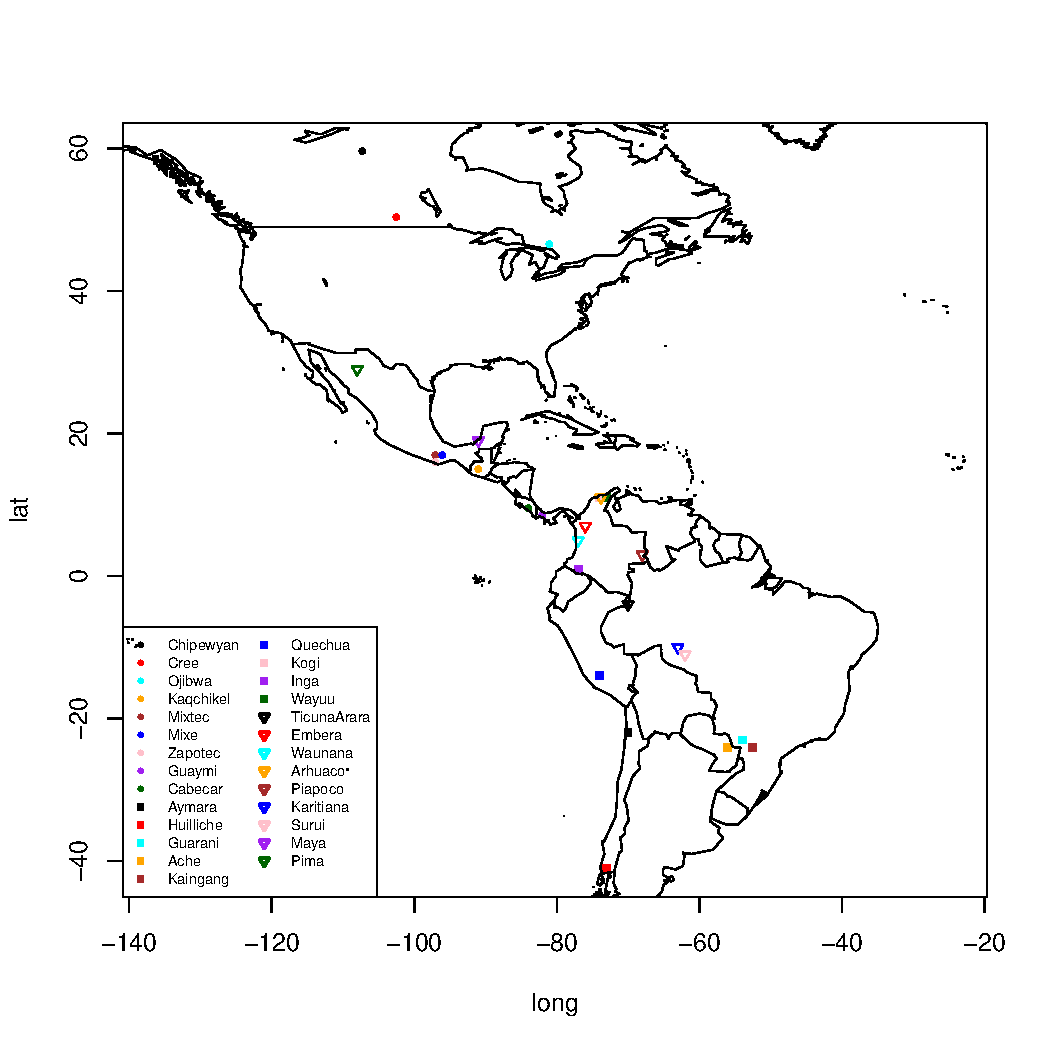
\includegraphics[scale=1]{map.pdf}
\caption{Origine géographique des indiens d'Amérique}
\end{center}
\end{figure}

\end{enumerate}


\section{Régression}
%Le problème c'est qu'on est incapable de trouver les coefficients de la régression de la longitude car le nombre de marqueurs génétiques (5709) est beaucoup plus grand que le nombre d'individus (494). C'est pourquoi on régressera la latitude et la longitude avec les scores de l'ACP faite les marqueurs génétiques. 
%
%À refaire (avec le cours) avec une démonstration mathématique.

La régression n'est pas effectuée par R : les coefficients $(\hat{\beta_{j}})_{0 \leq j \leq p}$ renvoyés valent $NA$ (Not available). Le problème est la non-unicité de la régression.

Lorsque $n \geq p+1$, alors $X^{T} X$ est inversible, et l'unique solution de la régression est :
\begin{displaymath}
\hat{\beta} = (X^{T} X)^{-1} X^{T} y
\end{displaymath}
Par contre, ici, $n < p+1$.
D'où :
\begin{eqnarray*}
rang(X^{T} X) & \leq & rang(X) \\
& \leq & n \\
& < & p+1
\end{eqnarray*}
$X^{T} X$ est une matrice carrée de taille $p+1$, de rang strictement inférieur à $p+1$. Donc $X^{T} X$ n'est pas inversible, et la solution de la régression n'est pas unique.


\section{ACP}
\begin{enumerate}
\setlength{\itemsep}{20pt}
\item[3.a)]
 Le principe de l'Analyse en Composantes Principales est de tirer parti de la corrélation entre les variables du problème pour expliciter un nombre réduit de nouvelles variables, combinaison linéaires des anciennes, qui permettent de modéliser correctement la variance de l'échantillon. Son intérêt majeur est donc de limiter le nombre de variables à étudier. Ici, réaliser une ACP permet ensuite de régresser les coordonnées géographiques.

 \item[3.b)]
 On réalise une ACP sur les données génétiques avec tous les individus. 
 On n'a pas besoin d'utiliser l'argument scale car les variables (les marqueurs génétiques) n'ont pas d'unités de mesures : les valeurs sont binaires. Il n'y a donc pas besoin de mettre ces variables sur une même échelle.

\begin{figure}[!h]
\begin{center}
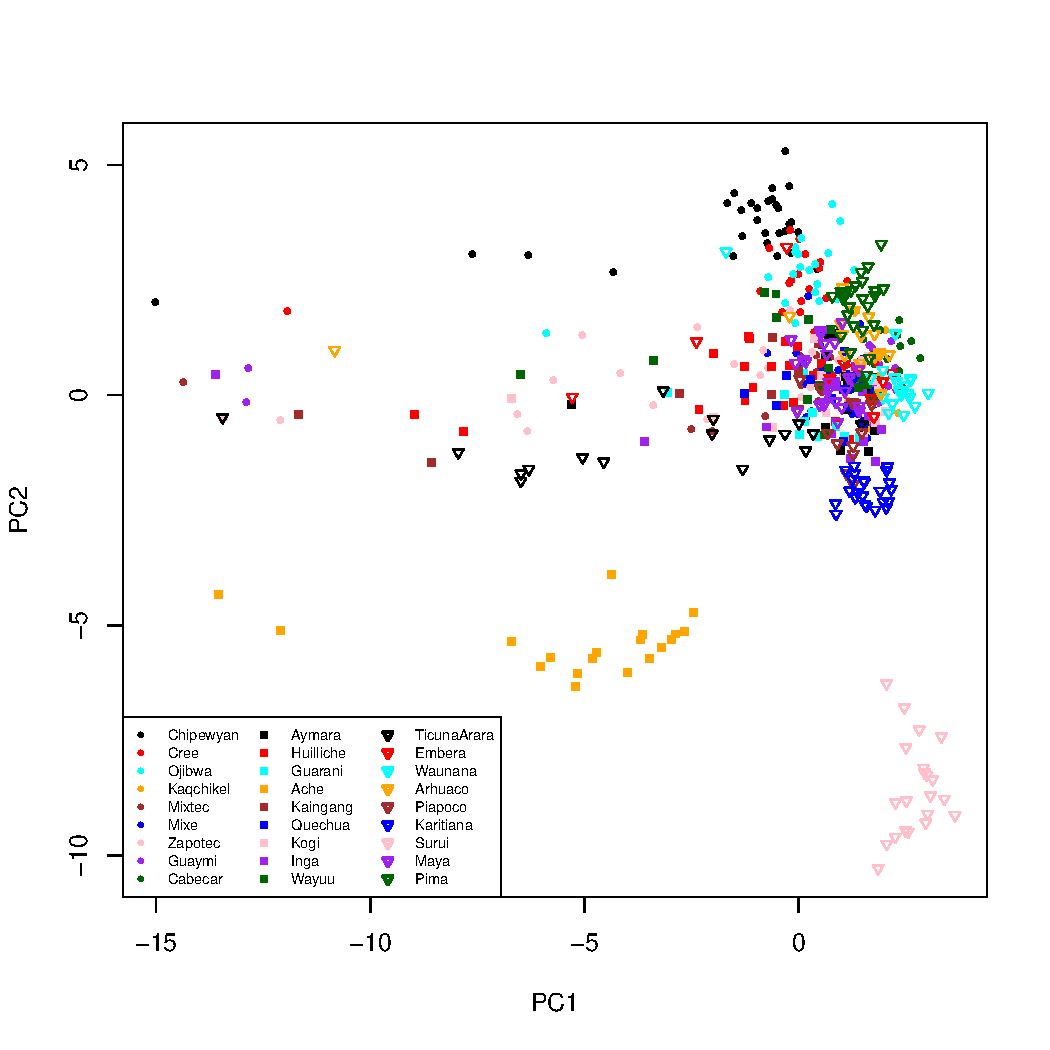
\includegraphics[scale=1]{acp12.pdf}
\caption{Les populations projetées sur les 2 premières PC}
\end{center}
\end{figure}

En considérant les 2 premiers axes de l'ACP, les individus qui sont facilement identifiables sont les Surui et les Aches. En effet, ils sont relativement éloignés de l'origine, et les vecteurs associés ne sont pas colinéaires et de même sens (cf. figure 2). Cependant, en observant la figure 1, on s'aperçoit que les localisations associées sont relativement proches. Ainsi, les Surui et les Aches se différencient bien génétiquement, mais ces différences ne sont pas corrélées à une origine géographique différente. En régressant les coordonnées géographiques selon les axes de l'ACP, on s'aperçoit effectivement que le premier axe est indépendant de la localisation (cf. question 4.a)).
\pagebreak
\begin{figure}[!h]
\begin{center}
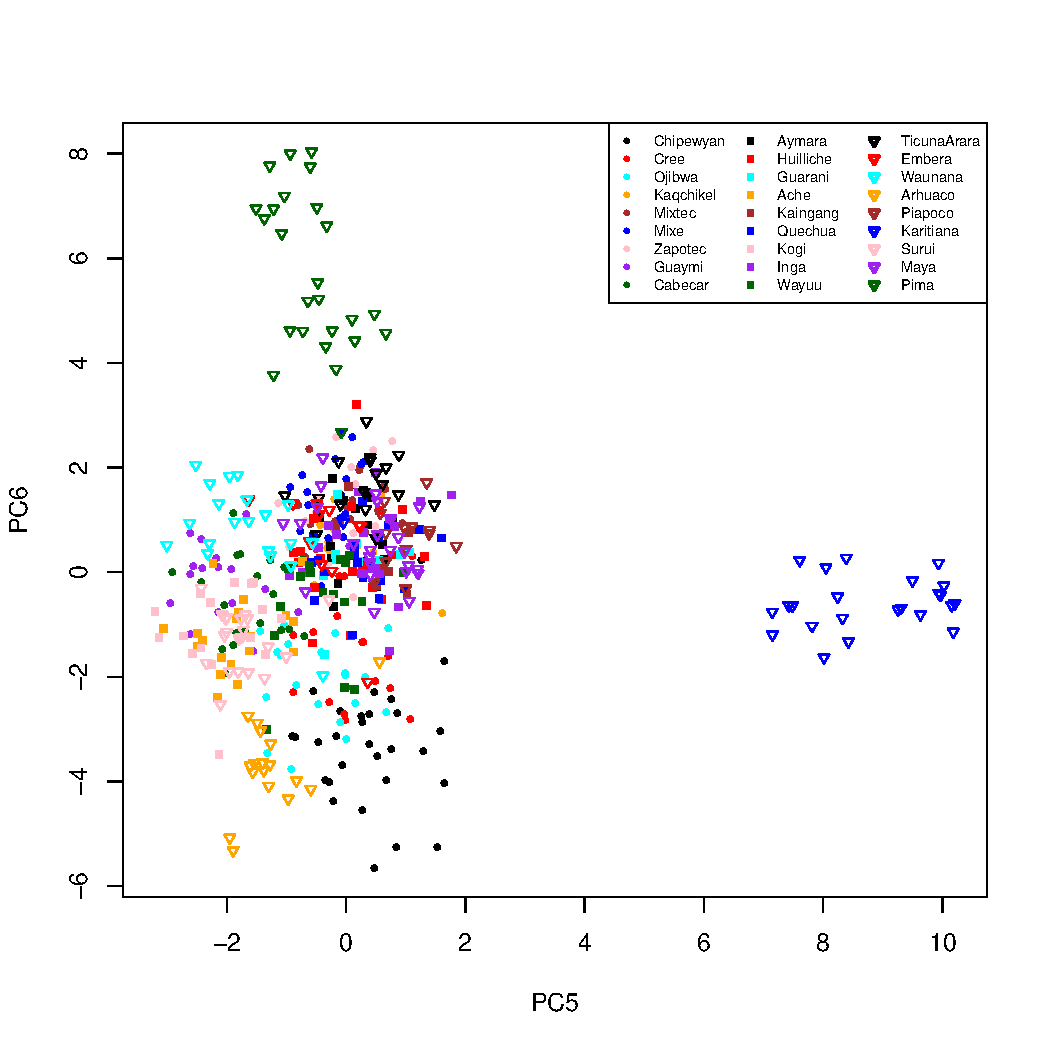
\includegraphics[scale=1]{acp56.pdf}
\caption{Les populations projetées sur les PC 5 et 6}
\end{center}
\end{figure}

Avec les axes 5 et 6, ce sont les Karitiana et les Pima qui sont facilement identifiables, d'autant plus que chacun des vecteurs associés est aligné sur un axe différent (cf. figure 3).

 \item[3.c)] 
 Le pourcentage de variance cumulée expliquée par les $2$ premières PC est de $3,57\%$. Ce pourcentage paraît relativement faible, mais il ne faut pas oublier que l'on part d'un très grand nombre de variables ($p = 5709$ marqueurs génétiques). En prenant deux variables de départ quelconques, on expliquerait en moyenne $2/p = 0.035\%$ de variance. On a donc réussi à expliquer $100$ fois plus de variance.
 
 En gardant les 250 premiers axes de l'ACP, on exprime $77 \%$ de la variance du jeu de données, en divisant par $20$ le nombre de variables.

\end{enumerate}

\section{PCR Principal Components Regression}

\begin{enumerate}
\setlength{\itemsep}{12pt}

\item[4.a)]
On régresse la latitude et la longitude en utilisant comme prédicteurs les scores des 250 premiers axes de l'ACP. On observe que le premier axe n'influe pas sur la localisation en dépit du fait qu'il maximise la variance des variables. Dans les deux régressions, la p-valeur associée est très grande (respectivement $44\%$ et $23\%$ pour la régression de la longitude et de la latitude) par rapport aux p-valeurs des autres axes. Donc il y a de forte chance que le coefficient de régression associé au premier axe soit nul. 

\item[4.b)]
On affiche sur une carte les coordonnées spatiales régressées pour chaque individu (cf. figure 4). Cette carte donne une image trop optimiste de la capacité à retrouver l'origine géographique d'un individu à partir de ses marqueurs génétiques. En effet, on a considéré uniquement l'erreur de régression, et pas l'erreur de prédiction. On fait donc face à un problème d'overfitting : on cherche trop à "coller" aux données, autrement dit on régresse aussi le bruit.

Par ailleurs, il est illusoire de croire que tous les marqueurs génétiques (ou tous les axes de l'ACP) sont corrélés à l'origine géographique. On l'a vu : le premier axe de l'ACP est indépendant de l'origine géographique.


\begin{figure}[!h]
\begin{center}
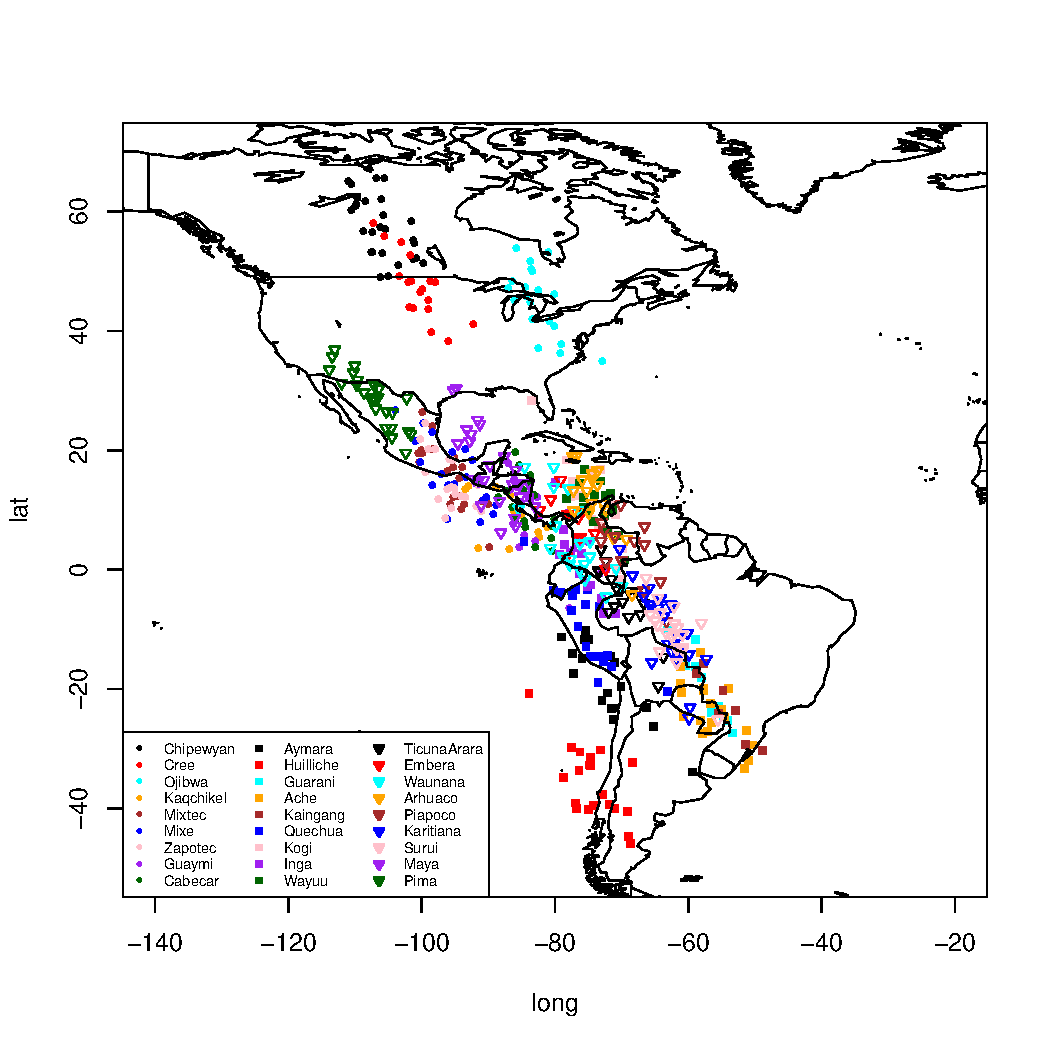
\includegraphics[scale=1]{map_acp.pdf}
\caption{Régression des coordonnées spatiales avec les 250 premiers axes de l'ACP}
\end{center}
\end{figure}

\item[4.c)]
Pour le modèle précédent (250 axes), l'erreur moyenne en termes de distance est de $641$ km. Etant donnée la complexité de l'histoire humaine (migrations, brassages génétiques), et à l'échelle du continent américain, c'est une erreur relativement faible. Mais n'oublions pas que le problème d'overfitting n'est pas encore réglé, et que l'erreur finale sera donc plus grande.

Ce résultat nous permet néanmoins d'affirmer qu'il n'est en général pas possible de prédire très précisément l'origine géographique d'un individu à partir de ses marqueurs génétiques. Sur la carte (figure 4), on remarque en particulier que les coordonnées régressées des individus en provenance de tribus d'Amérique Centrale sont fortement mélangées, on ne peut donc pas reconstituer les tribus d'origine de ces individus.

\end{enumerate}

\end{document}

% TODO : parler du scrum master
